\documentclass[a4paper, 12pt]{report}
%\setcounter{chapter}{1}
\renewcommand\thesection{\arabic{section}}
\renewcommand{\contentsname}{Cuprins}
\renewcommand{\figurename}{Figura}
\renewcommand{\tablename}{Tabel}

\setcounter{tocdepth}{6}
\setcounter{secnumdepth}{6}

\usepackage{url}
\usepackage{hyperref}
\usepackage[backend=bibtex, style=numeric, citestyle=numeric, backref=true ,sorting=none]{biblatex}
\addbibresource{bibliography.bib}

\usepackage{indentfirst}
\usepackage[nobottomtitles*]{titlesec}

\usepackage{graphicx}
\usepackage[center]{caption}
\usepackage{caption}
\usepackage{subcaption}
\usepackage[export]{adjustbox}
\graphicspath{ {./images/} }



\usepackage[margin=3.2cm]{geometry}
%\usepackage[none]{hyphenat}

\usepackage{mathtools}

\usepackage{listings}
\usepackage{color}
\usepackage{float}

\definecolor{codegreen}{rgb}{0,0.6,0}
\definecolor{codegray}{rgb}{0.5,0.5,0.5}
\definecolor{codepurple}{rgb}{0.58,0,0.82}
\definecolor{backcolour}{rgb}{0.96,0.96,0.96}

\lstdefinestyle{mystyle}{
	backgroundcolor=\color{backcolour},   
	commentstyle=\color{codegreen},
	keywordstyle=\color{blue},
	numberstyle=\tiny\color{codegray},
	stringstyle=\color{codepurple},
	basicstyle=\fontsize{10}{10}\selectfont\ttfamily,
	breakatwhitespace=false,         
	breaklines=true,                 
	captionpos=b,                    
	keepspaces=true,                 
	numbers=left,                    
	numbersep=2pt,                  
	showspaces=false,                
	showstringspaces=false,
	showtabs=false,                  
	tabsize=2
}

\lstset{style=mystyle}

\usepackage{pythonhighlight}

\usepackage{fontspec} % -> LuaLatex
\setmainfont{UT Sans}

\usepackage{setspace}
\setstretch{1.1} % 

\begin{document}
	
	\begin{titlepage}
	
	\vspace*{-3cm}
	\hspace{-2cm}
	
\includegraphics[width=0.8\linewidth]{./images/Logo-UT-MI-SPOT-RO}

	\begin{center}
		\Huge
		
		\vspace{2cm}
		
		\textbf{Lucrare Dizertație}
		
		\vfill
				
		\Large
		\begin{tabular}{ll}
			\textbf{Autor:}&Hanganu Bogdan\\
			\textbf{Coordonator:}&Lect. Univ. Băicoianu Alexandra
		\end{tabular}
		
		\vfill
		
		\Large
		Brașov\\
		Iulie 2022
        
	\end{center}
\end{titlepage}
	\begin{titlepage}
	
	\vspace*{-3cm}
	\hspace{-2cm}
	
\includegraphics[width=0.8\linewidth]{./images/Logo-UT-MI-SPOT-RO}
	
	\begin{center}
		\Huge
		
		\vspace{2cm}
		
		\textbf{Lucrare Disertație}
		
		\vspace{1cm} 
		
		\LARGE Detectarea emoțiilor din perspective multiple
		
		\vfill
		
		\Large
		\begin{tabular}{ll}
			\textbf{Autor:}&Hanganu Bogdan\\
			\textbf{Coordonator:}&Lect. Univ. Băicoianu Alexandra
		\end{tabular}
		
		\vfill
		
		\Large
		Brașov\\
		Iulie 2022
		
	\end{center}
\end{titlepage}
	\newpage
	\tableofcontents
	\newpage
	\pagenumbering{arabic}
	\section{Abstract}	
	Această lucrare de disertație este elaborată în jurul problematicii identificării emoțiilor unei persoane. Utilizând metode de învățare automată, datele sunt înregistrate prin intermediul unor canale multiple (audio, video și text). Expresiile faciale, obținute prin intermediul canalului video, reflectă în mod intuitiv starea mentală a unei persoane, fiind una dintre cele mai bogate și importante forme de comunicare inter-umană. Tonalitatea vocii care se adresează în timpul comunicării ne poate oferi informații valoroase referitoare la starea de spirit. Mesajul care este transmis prin intermediul vocii, ne oferă informații referitoare la personalitatea individului, fiind de ajutor mai departe în procesul de analiză.
	Datele stocate sunt mai apoi prelucrate folosind tehnici de procesare specifice fiecărui canal. Pentru input-ul audio este folosită procesarea digitală de semnal, cu următoarele tehnici reprezentative: Transformata Fourier, Transformata Fourier pe termen scurt, Coeficienți Mels. Procesare de imagini pentru canalul video vine în adăugare cu: scalare de date, transformare imaginii în greyscale, iar pentru text este de menționat: tokenizare, lematizare. Fiecare bloc de date preprocesat în mod corespunzător canalului părinte, va trece mai departe prin pasul de recunoaștere cu ajutorul metodelor de învățare automată.
	În această lucrare au fost realizate o serie de experimente pentru: procesarea datelor, antrenarea modelelor de machine learning. Finalizarea acestor teste a avut ca urmare dezvoltarea aplicației "Multimodal Emotion Detection" care să vină în sprijinul procesului de intervievare.
	\clearpage
	
	\section{Introducere}
	Aplicația "Multimodal Emotion Detection" are ca audiență persoanele care doresc să facă o analiză a candidatului care a trecut printr-un proces de intervievare. Fiind scrisă în limbajul de programare Python, permite o manevrare concisă a datelor inregistrate, care pot fi mai apoi vizualizate de către utilizator prin intermediul framework-ului GUI (Graphical User Interface) QT (pronunțat "cute"). 
	
	În cadrul lucrării, se propune recunoașterea emoțiilor utilizatorului într-un mod inteligent, utilizând tehnici și metode de Machine Learning si Deep Learning. Aceste două procedee sunt subcategorii ale domeniului numit inteligență artificială, domeniu care a început să se modeleze în funcție de nevoile oamenilor.
	
	Dezvoltarea rapidă a inteligenței artificale, "Big data science" și a tehnologiei "Block chain" a provocat multiple schimbări în structura socială umană. În majoritatea proceselor unde este nevoie de interacțiune umană, se implementează automatizări care să sporească eficiența, să folosească resursele umane, software și hardware în mod cât mai eficace. La nivel industrial, sistemele automatizate inteligente sunt deja folosite in uzine, frabici, având rolul de a asigura în permanență buna funcționare a întregului ansamblu. Atât eficiența cât și performanțele acestor sisteme sunt motivate de către costul redus de mentenanță. La un nivel mai aproape de către utilizatori, putem realiza că inteligența artificială a început tot mai des să facă parte din viața de zi cu zi, ajungând în stadiul să devină indispensabil oamenilor.
	
	În zilele noastre, interacțiunea dintre oameni și I.A. este în continuă creștere, ajungand să intre treptat în viața noastră de zi cu zi. De la asistenți virtuali (care au rolul de a sprijini utilizatorul prin intermediul interpretării comenziilor vocale), până la reclame personalizate, aceste sisteme inteligente interacționează din ce în ce mai mult cu ființe umane. Deoarece este un subiect în care interesul este unul foarte crescut, relația între om și mașinăria inteligentă poate să ajungă la un nivel mai inalt, prin integrarea cu emoțiile utilizatorului. Acesta este un domeniu crucial de cercetare, oferind diverse oportunități și aplicări pentru oameni.
	
	Astfel, în următorul capitol va fi explicat despre fiecare din cele trei tipuri de recunoaștere a emoției utilizate, precum și modul în care acestea interacționează cu utilizatorul. Vor fi prezentate exemple de alte categorii a recunoașterii de emoții, care nu au fost încadrate în această lucrare, precum și aplicațiile care sunt deja în domeniul comercial și sunt utilizate.
	
	\clearpage
	\section{Recunoașterea emoțiilor}
	Un aspect cheie în această sferă care să sporească parteneriatul între om și mașină este dat de înțelegerea emoțiilor umane. Emoția este un factor important atât în comunicarea verbală, cât și în comunicarea nonverbală (gesticulare, expresiile corpului). Identificarea stărilor unei persoane poate ajuta o mașină să înțeleagă intențiile utilizatorului, în scopul de a-i oferi o interacțiune mai potrivită. Printe primele studii care au fost făcute pentru integrarea sistemelor inteligente cu emoțiile umane, aceastea s-au reflectat în identificarea emoțillor prin voce, deoarece comunicarea verbala este una dintre cele mai rapide forme de socialiare, cu cel mai mare impact in istorie.
	
	Fiind una dintre cele mai consacrate aptiduni prin care o ființă inteligentă s-a putut diferenția și avansa în lanțul trofic, comunicarea verbală reprezintă un semnal complex, în care sunt transmise informații referitoare la mesaj, legate de emițător precum și de emoțiile transmise de acesta. Fiind o serie complexa, capacitatea sistemului care face identificarea emotiilor trebuie sa fie pe măsură, pentru a analiza cu acuratețe starea subiectului, oferindu-i astfel o experiență cât se poate de autentică. Nu numai atât, utilizând o astfel de recunoaștere, poate ajuta la crearea unor interfețe usor navigabile("Recunoașterea emoțiilor prin vorbire este deosebit de utilă pentru aplicațiile din domeniul interacțiunii om-mașină deoarece ajută la crearea unor interfețe usor de utilizat"\cite{emotion_recognition_survery}).
	
	Deoarece semnalul audio conține și alte informații precum emoția transmisă de către emițător, algortimul de recunoaștere a emoțiilor umane prin extragerea trăsăturilor acustice capturate în vorbire, devine "baza pentru realizarea unei interacțiuni om-calculator mai armonioasă și mai eficientă, având o mare importanță în cercetare, precum și aplicativă"\cite{audio_emotion_recognition0}.
	
	În cadrul aplicației, vocea utilizatorului (semnalul audio) este folosită în doua contexte. Primul este dat de către identificarea emoțiilor candidatului pe baza a diferite trăsături acustice depistate din voce iar al doilea de către identificarea cuvintelor rostite, pentru a putea fi transformate în text. Deoarece în aplicatie identificarea textului (speech-to-text) este utilizat prin intermediul unor apeluri de tip API Rest la functionalitățile oferite de către Google, accentul se va pune pe prima utilizare în lucrare. Emoțiile care pot fi identificate în cadrul acestei recunoașteri sunt următoarele: furie, dezgustare, frică, fericire, tristețe, surprindere, neutral.
	
	Seviciului oferit de către Google pentru recunoașterea textului \cite{google_speech_to_text} este folosit cu scopul de a facilita identificarea personalității și a emoției transmise în urma interviului de către utilizator. Recunoașterea emoțiilor din text este în mod fundamental o problemă de clasificare pe baza conținutului, care include noțiuniuni de procesare de text (NLP, acronim de la "natural language processing"), precum și din domeniul deep learning. Modelul utilizat pentru acest tip de predicție este "The Big Five personality traits"\cite{big_five_personality_wiki}. 
	
	\begin{figure}[h]
		\begin{center}
			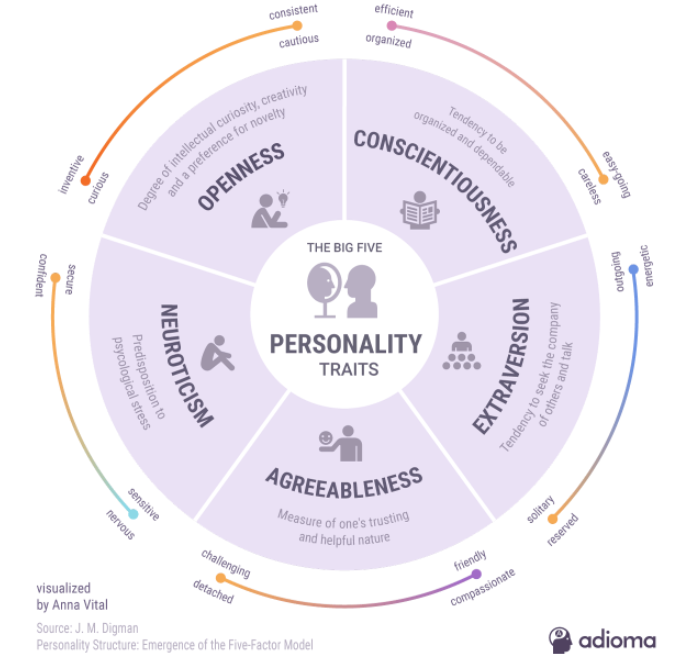
\includegraphics[scale=0.7]{images/ocean.png}
		\end{center}
		\caption{Cele cinci mari trăsături de personalitate\newline
			\hspace{\linewidth}https://blog.adioma.com/5-personality-traits-infographic/}
		\label{fig:ocean}
	\end{figure}
	
	În zilele noastre, se consideră că există 5 categorii de personalități (Figura \ref{fig:ocean}), având acronimul OCEAN. Mai jos, vom prezenta aceste personalități de bază:
	\begin{itemize}
		\item Openness (Deschidere): această trăsătură prezintă caracteristici precum imaginația și perspicacitatea. Oamenii care au punctat mai mult în această trăsătură tind să aibe o arie mai mare de interese. Sunt curioși de fire, dornici să dobândească aptitudini noi și să se bucure de orice experiență acumulată.
		
		\item Conscientiousness (Conştiinciozitate): printre caracteristicile de baza ale acestei trăsături, putem include un nivel ridicat de atenție, control bun al impulsurilor și comportamente care coduduc spre îndeplinirea obiectivelor. Oamenii care se încadrează acestei categorii tind să fie mai organizați și atenți la detalii. Ei planifică din timp, se gândesc la modul în care comportamentul lor îi afectează pe alții și sunt atenți la termenele limită.
		
		\item Extraversion (Extraversie): se caracterizează prin excitabilitate, sociabilitate și cantități mari de expresivitate emoțională. Oamenii care au un nivel ridicat de extraversie tind să capete energie în situații sociale. A fi în preajma altor persoane îi ajută să se simtă plini de energie și entuziasm.
		Oamenii care au un nivel scăzut de extraversie (sau introvertiți) tind să fie mai rezervați și au mai puțină energie în mediile sociale. În urma evenimentelor sociale se pot simți extenuați, iar introvertiții necesită adesea o perioadă de singurătate și tăcere pentru a își putea "reîncărca bateriile".
		
		\item Agreeableness (Agreabilitate): pentru această personalitate, sunt incluse atribute precum încrederea, altruismul, bunătatea, afecțiunea și alte comportamente pro-sociale. Oamenii cu grad ridicat de agreabilitate tind să fie mai cooperativi, în timp ce aceia care au punctat mai slab pentru acest atribut, tind să fie competitivi și uneori chiar manipulativi.
		
		\item Neuroticism (Nevrotism): este un atribut caracterizat prin tristețe, melancolie și inconsevcență emoțională. Persoanele care au această trăsătură au tendința de a experimenta schimbări de dispoziție, anxietate, iritabilitate și tristețe. Aceia care au punctat scăzut în acest caz, tind să fie mai stabili și rezistenți emoționali.
	\end{itemize} 
	
	Nu în cele din urmă, dupa procesul de recunoaștere a trăsăturilor și emoțiilor transmise din voce, mai apoi interpretate în mod contextual prin procesare de text, urmează recunoașterea emoțiilor din cadrul expresiilor faciale. Pentru a putea fi în stare să facem o astfel de analiză, este nevoie identificarea unui chip uman (în engleză "face detection"). Pentru a facilita acest proces, prin intermediual camerei web care ne oferă flux de date video, biblioteca OpenCv\cite{open_cv} ne oferă suport pentru mijloace de identificare a fețelor candidaților. Având acest rezultat intermediar, este posibilă recunoașterea emoțiilor pe baza expresiilor faciale. Principalele stări emotive din cadrul fluxului video sunt aceleasi ca cele din audio.
	
	Făcând un ansamblu al componentelor descrise mai sus, acestea se unifică în ceea ce vom numi "Modulul de intervievare". În cadrul acestui modul, predicțiile pentru componentele audio și video sunt făcute live, iar in cazul textului, este realizat la final pentru a avea o cantitate mai ridicată de date, obținânand astfel o predicție cât mai aproape de adevăr.
	
	Tipurile de identificare a emoțiilor utilizate și descrise mai sus sunt doar câteva modele existente prin care o aplicație/mașină inteligentă poate interacționa în mod personalizat cu utilizatorul. Printre alte tipuri care merită menționate se enumeră gesturile corpului (limbajul corpului), fiind un subiect mai puțin explorat. Chiar dacă este un aspect important al psihologiei umane, primule studii moderne au devenit populare debia în 1960. Probabil cea mai importantă lucrare publicată înainte de secolul al XX-lea a fost "Expresia emoțiilor la om și la animale", scrisă de Charles Darwin \cite{human_body_lang_darwin}.
	
	În acest domeniu, după o cercetare a pieței care construiesc software-uri în jurul predicției emoțiilor, putem considera aplicațiile menționate mai jos ca fiind similare cu cea prezentată în această lucrare:
	\begin{itemize}
		\item Noldus Solutions Emotion Analysis cu "FaceReader™" \cite{noldus}: este un software specilizat pe analizarea datelor de tip imagine (atât din video cât și statice). Este un sistem robust, capabil să recunoască un număr de proprietăți specifice în imaginile faciale, inclusiv cele șase expresii de bază sau universale: fericit, trist, furios, surprins, speriat și dezgustat.
		\item iMotions cu "Facial Expression Analysis" \cite{imotions}: este un software specializat atât în analiza imaginilor cât și a datelor biosenzoristice. Modulul oferă 20 de măsuri de expresie facială (unități de acțiune), 7 emoții de bază, repere faciale, indici comportamentali, cum ar fi orientarea capului și atenția.
	\end{itemize}
	
	Diferența pe care o aduce aplicația prezentată în lucrare ("Multimodal Emotion Detection") este reprezentată de capacitate recunoașterii în timp real a emoțiilor prin intermediul altor input-uri, precum și a feedback-ului constant. Un alt aspect important prin care se diferențiază aplicația în cauză este dat de "Modulul de vizualizare a raportului", prin care se poate vedea la fiecare segment de date, textul care a fost spus, emoțiile prezise din input-ul audio, video, cât și o spectogramă pentru intervalul selectat de date în care s-a efectuat predicția.
	
	Gama de public cărui este adresată această aplicație este reprezentată în general de persoanele care trec prin procesul de intervievare. Dar asta nu înseamnă că recunoaștere emoțiilor se limitează la această aplicativitate. Mai jos sunt listate o serie de utilizări:
	\begin{itemize}
		\item Marketing personalizat: un studiu realizat de OneSpot Research a arătat că în proporție de 88\% dintre consumatorii chestionați au declarat că un conținut mai personalizat îi face să se simtă mai bine cu privire la un anumit brand.
		\item Diagnostic medical: o aplicativitate în care poate sprijinii medicii cu diagnosticarea afecțiunilor nevrotice precum depresia sau demența, utilizând analiza vocală
		\item Educație: diferite software-uri didactice în variantă prototip au fost elaborate pentru a se acomoda la emoția copiilor. Când copilul exprimă frustrare pentru că o sarcină este prea simplă sau dificilă, programul se adaptează astfel încât sarcina să se schimbe într-o formă mai adecvată.
	\end{itemize}
	
	În urmatorele capitole, vom trece printr-o inițiere în inteligența artficială, procesare digitală de semnal, procesare de imagini și text. Având aceste cunoștiințe asimilate, următoarele subiecte propuse care vor fi comentate se vor afla în sfera tehnologiilor utilizate, fără de care nu s-ar fi putut crea aceste teste, precum și aplicația "Multimodal Emotion Detection". 
	\clearpage
	
	\section{Noțiuni teoretice}
	\subsection{Inteligența artificială}
	David Fogel a definit inteligența ca fiind "abilitatea unui sistem de a se adapta astfel încât să își poată îndeplini scopurile cu succes". Astfel, o mașinărie programată și dotată cu inteligență artificială este un sistem complex capabil să facă decizii, fără nevoia intervenției unei persoane, simulând inteligența umană. Perturbarea funcționării unui astfel de sistem poate altera fluxul evenimentelor în luarea deciziilor, ajungând astfel la rezultate nejustificabile. Principalele subcategorii ale I.A. sunt: machine learning (învățare automată) și deep learning (învățare profundă).
		
	\begin{figure}[h]
		\begin{center}
			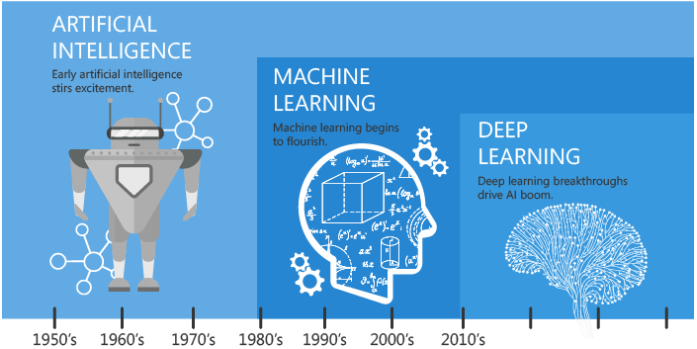
\includegraphics[scale=0.8]{images/AI_ML_DL.png}
		\end{center}
		\caption{Dezvoltarea inteligenței artificiale\newline
			\hspace{\linewidth}https://towardsdatascience.com/artificial-intelligence-vs-machine-learning-vs-deep-learning-2210ba8cc4ac/}
		\label{fig:AI_ML_DL}
	\end{figure}
	
	Așa cum se observă în Figura \ref{fig:AI_ML_DL}, putem afirmă că inteligența artificială este un termen mai vast care cuprinde celelalte două subcategorii. Aplicațiile care utilizează acest tip de tehnologie imită funcțiile cognitive pe care oamenii le asociază cu mințile umane, cum ar fi învățarea sau rezolvarea anumitor probleme.
	
	Învățarea automată (machine learning) înglobează algoritmii clasici pentru diferite tipuri de sarcini, precum regresia sau clasificarea. Acești algoritmi sunt dependenți în permanență de datele utilizate în procesul antrenării. Cu cât sunt mai multe date și cu cât aceste date sunt mai relevante pentru problema care încearcă să se soluționeze, randamentul acestora va crește. Antrenarea lor reprezintă cel mai important pas, deoarece în acest proces, se presupune minimizarea funcției de eroare (loss function). Rolul acesteia este de a stabili valorile de adevăr între ce a fost prezis, și adevărata clasă a datelor respective. În raport cu răspunsul funcției de eroare în cauză, anumite valori denumite greutăți (weights) vor fi actualizate.
	
	În învățarea automată există două categorii de date din care se poate învăța: date etichetate și date neetichetate. În prima categorie, atât parametrii de intrare cât și cei de ieșire sunt într-o formă ușor de citit pentru mașină, fiind nevoie de o cantitate mare de timp pentru a putea eticheta. În cazul datelor neetichetate, este nevoie de o soluție mai complexă pentru a putea utiliza acele informații. Astfel, reies la suprafață trei tipuri de învățare în machine learning:
	\begin{itemize}
		\item Învățare supervizată: este una din cele mai de bază tipuri de învățare automată. Chiar dacă este antrenat cu date etichetate, acest gen de învățare este unul foarte puternic. Se folosește un set de date (sau o parte din acest set de date, în general referindu-ne ca set de antrenare), care servește algoritmului cu scop de pregătire, iar alt set de date pentru a testa performanțele modelului.
		\item Învățare nesupervizată: principalul avantaj al acestei categorii este capacitatea algoritmilor de a lucra cu seturi de date neetichetate, eficientizând timpul programatorului. Permit astfel algoritmilor să exploreze și să găsească diferite șabloane și asocieri în seturile de date.
		\item Învățare prin "întărire" (reinforcement): se inspiră direct din modelul în care ființele umane învață din experiențele din viața de zi cu zi. Dispune de un algoritm care se îmbunătățește pe sine și învață din situații noi folosind o metodă de "încearcă și greșește" (în engleză trial and error). Rezultatele favorabile sunt încurajate sau "întărite", iar rezultatele greșite sunt descurajate sau "pedepsite".
	\end{itemize}
	
	Referitor la Figura \ref{fig:AI_ML_DL}, se poate constanta că machine learning este un domeniu destul de îmbătrânit, care încorporează metode și algoritmi, precum: Naive Bayes Classifier, Support Vector Machine, Random Forest. 

	Recent, în industria inteligenței articiale, a apărut conceptul de deep learning, care asamblează rețele artificiale neurale cu mai multe straturi. Deep learning poate fi definit ca un subset al învățării automate, care încearcă rezolvarea problemelor mai complexe prin găsirea unor diferite șabloane (pattern-uri) în date, acestea pentru oameni fiind insesizabile cu ochiul liber.

	Avantajul pe care îl aduc aceste tipuri de rețele față de cele tradiționale, este dat de eliminarea necesității de a extrage caracteristici (feature) din cadrul setului de date. Rezultatul extragerii caracteristicilor din setul de date definește o reprezentare abstractă a datelor. Acest proces este de obieci destul de complicat, care necesită cunoștințe detaliate în aria specifică a problemei care se încearcă soluționarea. Pasul extragerii trebuie revizuit de multiple ori, testat și rafinat pentru a obține rezultate optime.
	
	\clearpage
	
	\begin{figure}[h]
		\begin{center}
			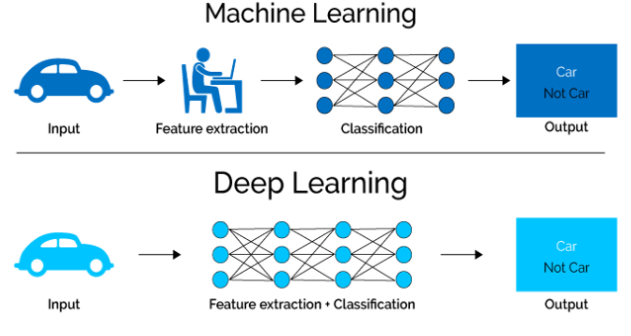
\includegraphics[scale=0.7]{images/ML_DL.png}
		\end{center}
		\caption{Analogie învățare automată și învățare profundă\newline
			\hspace{\linewidth}https://www.researchgate.net/figure/Comparison-between-ML-and-Dl-algorithm\_fig5\_344628869/}
		\label{fig:ML_DL}
	\end{figure}

	Pe de altă parte, în Figura \ref{fig:ML_DL}, se poate observa cum în cazul învățării profunde, pasul de extragere a caracteristicilor nu mai este necesar să fie executat de către programator, ci devine parte în procesul de antrenare a rețelei artificiale. Datele sunt brute și abstractizate astfel încât să poată fi memorate de diversele straturi ale algoritmului inteligent. Această reprezentare comprimată a datelor de intrare este utilizată pentru a construi rezultatul.

	Cu ajutorul rețelelor neurale profunde, acestea au făcut posibilă înțelegerea a seturilor de date complexe, precum semnalul audio reprezentând vocea umană, expresiile faciale și textul asociat cu fraze. Datele de antrenare folosite (care vor fi prezentate în capitolele următoare), sunt etichetate, făcând astfel posibilă identificare emoțiilor și a personalității candidatului. În secțiunea următoare, vom prezenta în mod minimalist modelele utilizate în aplicație:
	\begin{itemize}
		\item Rețele neurale convoluționale
		\item Rețele neurale recurente
	\end{itemize} 

	\clearpage
	\subsubsection{Rețele neurale convoluționale}
	O rețea neurală convolutională este un de algoritm inteligent care face parte din clasa modelelor deep learning. În general folosite în vederea artificială (computer vision), CNN (convolutional neural network) primește ca date de intrare, în majoritatea cazurilor, imagini (sau date care au fost structurate sub forma imaginilor), iar în urmă diferitelor operațiuni, se vor găsi pattern-uri în datele de antrenare, nevizibile unei persoane în mod natural. Sunt distinse printre alte tipuri de modele datorită performanțelor ridicate cu date care provin din: imagini, vorbit 	sau semnal audio.
	
	Din punct de vedere structural, o rețea neurală convolutională este alcătuită din următoarele componente:
	\begin{itemize}
		\item \textbf{Date de intrare}: cum este menționat mai sus, input-ul poate să provină din mai multe categorii, având și canale diferite de culori. Nu există o limită privind dimensiunea datelor, deoarece, scopul întregului proces este de a reduce dimensionalitatea, păstrând datele într-o formă compresată, fără pierderi de informații.
		\item \textbf{Strart(uri) de convoluție}: este elementul de bază al unei astfel de rețele, fiind locul în care majoritatea calculelor au loc. În funcție de dimensionalitatea datelor (matrici 2d sau 3d), va avea loc operația de convoluție, cu ajutorul unor măști (kernel). În urma acestui proces, se vor extrage anumite trăsături importante din cadrul datelor de intrare, care vor ajuta în determinarea apartenenței la o anumită clasă. De exemplu, printr-o speculație, putem considera din Figura \ref{fig:cnn}, în urma unui proces de convoluție, că se poate determina dacă piciorul mamiferului este sau nu al unei zebre. În urmă acestui proces, în funcție de numărul filtrelor, pasul (stride) și padding, se obțin hărți ale caracteristicilor (feature maps).
		\item \textbf{Strat(uri) de pooling}: au rolul de a reduce substanțial dimensiunea spațială, scăzând cantitatea de parametrii utilizați pentru calcule în rețea. Totodată, poate controla și "supra-adaptarea" (overfitting) rețelei. Printre tipurile de straturi de pooling, putem menționa următoarele:
		\begin{itemize}
			\item \textbf{Max pooling}: fiind cea mai comună abordare, deoarece oferă cele mai bune rezultate, max pooling va selecta elementul maxim din harta caracteristicilor (porțiunea filtrată de către mască)
			\item \textbf{Average pooling}: cum reiese și din nume, va selecta valoare medie din porțiunea filtrată de mască
		\end{itemize}
		\item \textbf{Strat(uri) de conectare}: sunt folosite cu scopul conectării neuronilor către stratul de ieșire, unde în funcție de valorile ponderilor fiecărui neuron în parte, se va putea face calculul posibilității apartenenței la o anumită clasă
	\end{itemize} 
	
	\clearpage
	\begin{figure}[h]
		\begin{center}
			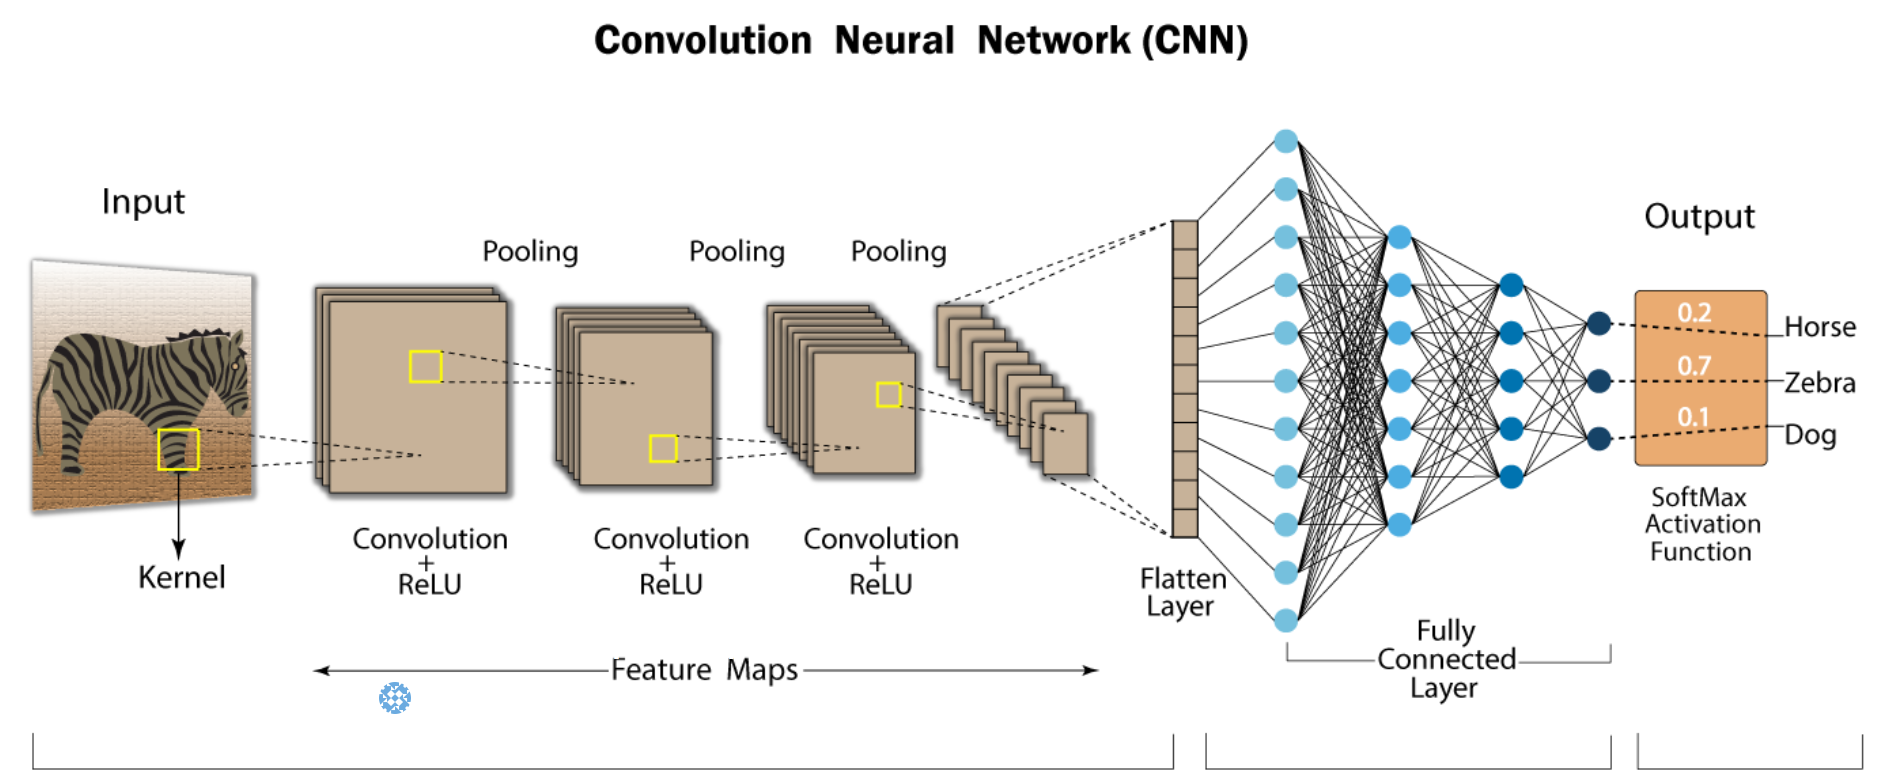
\includegraphics[scale=0.29]{images/cnn.png}
		\end{center}
		\caption{Rețea neurală convoluțională\newline
			\hspace{\linewidth}https://developersbreach.com/convolution-neural-network-deep-learning/}
		\label{fig:cnn}
	\end{figure}
	
	Împreună cu informațiile pe care le-am dobândit în urmă prezentării legate de rețelele neurale convolutionale, putem comenta asupra Figurii \ref{fig:cnn}. Din datele folosite pentru antrenare, filtrele aplicate succesiv ne vor ajută să găsim caracteristici. Transmise mai departe către stratul conectat, se va putea face interpretarea rezultatului, în funcție de gradul de apartenența la fiecare clasă în parte. Rezultatul va fi exprimat în procentaj, iar output-ul cu procentajul cel mai ridicat va exprima clasa decisă.
	\clearpage
	\subsubsection{Rețele neurale recurente}
	% Diacritice
	Retelele neurale recurente sunt un tip robust de retea neurala, folositoare pentru procesarea datelor secventiale, ordinea lor avand importanta. Derivate din retelele cu propagare inainte (feedforward), RNN-urile (recurrent neural network) prezinta un comportament asemanator cu cel al creierului uman.
	
	La fel ca ceilalti algoritmi de deep learning, retelele neurale recurente sunt relativ vechi, fiind conceputa in 1980, dar doar in ultimii ani a fost descoperit cu adevart potentialul acestora. Cresterea in puterea computationala, accesul la cantitati masive de date pe care le putem utiliza si aparitia straturilor cu memorie lunga pe durata scurta (long short-term memory), au adus RNN-urile in prim plan.
	
	Dupa cum mentioneaza Lex Fridman ("Ori de cate ori exista o secventa de date temporale, unde continutul spatial este mai important decat cel al fiecarui cadru individual"), retelele neurale recurente au oferit suport pe parcursul lucrarii pentru predictia datelor cu stransa legatura temporala. Aceste retele si-au indeplinit scopul in aplicatia "Multimodel Emotion Recognition" deoarece atat datele audio cat si cele video depinde de ordinea lor in timp.
	
	Datele secventiale sunt doar date ordonate in functide de un anumite criteriu. Spre exemplu, putem mentiona ca date secventiale datele financiare sau chiar secventa de ADN. Cele mai populare date secventiale sunt reprezentate de catre seria temporala, in care sunt enumerate in ordine cronologica. Datele provenite din vorbit, care sunt utilizate in aplicatie pentru a prezice emotia, sunt adevate acestei retele datorita sortarii cronologice standard.
	
	Pentru a intelege arhitectura acestor retele, trebuia mai intai sa avem cunostinte referitoare la mecanismul utilizat de aceasta retea, propagarea inainte. Intr-o retea neurala feed-forward, informatiile se misca doar intr-o singura directie: de la stratul de intrare, prin straturile ascunse, pana la nivelul de iesire. Informatia se deplaseaza direct prin retea si nu atinge acelasi un neuron de doua ori. Retelele simple nu au niciun mecanism de memorare, cu privire la intrarea pe care o primesc, fiind slabe in a prezice ce urmeaza. Intr-un RNN, informatia circula sub forma unei bucle. Cand se ia o decizie, se va evalua input-ul curent cat si ce a invatat din experientele anterioare.
	
	\begin{figure}[H]
		\begin{center}
			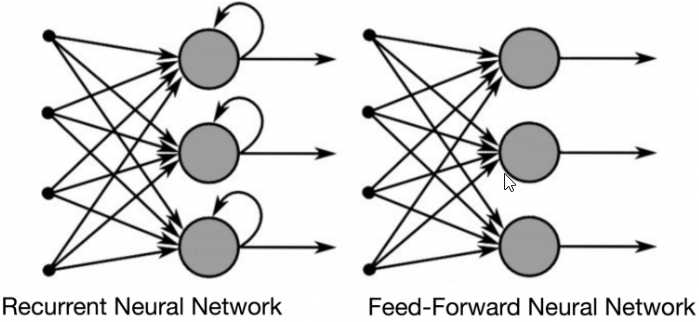
\includegraphics[scale=0.47]{images/fwd_recc.png}
		\end{center}
		\caption{Propagare recurentă și înainte\newline
			\hspace{\linewidth}https://builtin.com/data-science/recurrent-neural-networks-and-lstm/}
		\label{fig:fwd_recc}
	\end{figure} 

	In Figura \ref{fig:fwd_recc}, este ilustrata diferenta dintre fluxul de intratre intr-o reatea neurala recurenta si o retea cu propagare inainte.
	
	O retea neurala feed-forward atribuie, ca toti ceilalti algoritmi de deep learning, o matrice de ponderi care va fi aplicata asupra datelor de intrare, urmand mai apoi sa produca rezultatul. Totodata, va avea loc procesul de propagare inapoi (back propagation) petru actualizarea ponderiilor. 
	
	Propagarea inapoi este utilizata pentru a calcula gradientul unei functii de eroare in raport cu ponderile unei retele neurale. Algoritmul isi parcurge calea inapoi prin straturile retelei, calculand derivatele partiale a ponderilor. Aceasta tehnica este folosita pentru a reduce marjele de eroare in timpul antrenamentului.
	
	Mai jost sunt listate diferentele dintre o retea normala si una recurenta, in contextul celor doua propagari:
	\begin{itemize}
		\item Propagarea inainte: in acest pas, RNN-ul va inainta prin aplicarea ponderilor si pentru datele anterior procesate
		\item Propagarea inapoi: o astfel de retea modifica greutatile atat prin gradient descent cat si prin propagarea inversa in timp (back propagation through time)
	\end{itemize}

	Principalele neajunsuri in cazul acestor algoritmi au aparut datorita gradientului. Primul este denumit "Explozia gradientului" (Expploading Gradient) si apare in cazurile cand se asigneaza valori semnificativ de mari pentru ponderi. Aceasta este usor rezolvabila prin truncarea/plafonarea acestuia. A doua problema o reprezinta "Gradientul care dispare" (Vanishing Gradient), care apare atunci cand valorile gradientilor sunt prea mici, si modelul inceteaza sa invete ori o face intr-un timp prea mare. Pentru a rezolva aceasta problema, au fost introduse retelele cu LSTM (Long Short-Term Memory).
	
	Retelele LSTM sunt o extensie pentru RNN-uri, unde se extinde durata memoriei interne. Sunt folosite ca elemente de baza pentru straturile retelelor recurente. LSTM-urile asociaza alte inca un set diferit de ponderi folosit pentru a oferi un grad de importanta asupra datelor noi. In functie de aceste ponderi, datele noi vor putea impacta sau nu pe cele deja existente.
	
	Aceste straturi ofera suport retelelor recurente sa-si "aminteasca" input-urile pentru o perioada mai lunga de timp. Functionalitate lor este asemanatoare cu cea a unui calculator, avand capabilitati de citire, scriere sau stergere. Aceasta memorie poate fi privita precum o celula cu porti, care decide daca sa stocheze informatia, sa o stearga, in functie de importanta pe care trebuie sa o acorde.
	
	\clearpage
	\subsubsection{Antrenare utilizând procesorul grafic, CUDA}
	
	\clearpage
   \printbibliography
   \clearpage
	\begin{figure}[H]
		\begin{center}
			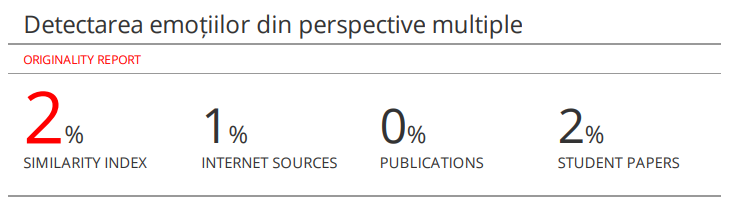
\includegraphics[scale=0.4]{images/plagiat.PNG}
		\end{center}
		\caption{Licență similaritate }
		\label{fig:sim}
	\end{figure} 	
\end{document}